
% Preamble
\documentclass[11pt]{article}

% Packages
\usepackage{amsmath}
\usepackage{mathtools}
\usepackage{ragged2e}
\usepackage [utf8]{inputenc}
\usepackage{blindtext}
\usepackage{wrapfig}
\usepackage{xcolor}
\usepackage {polski}
\usepackage{multicol}
\usepackage[a4paper, total={5.7in, 8in}]{geometry}
\usepackage{graphicx}
\usepackage{amstex}
\usepackage{csvsimple}
\usepackage{changepage}
\usepackage{enumitem}
\usepackage[english]{babel}
\usepackage{biblatex}
\usepackage{caption}
\usepackage{indentfirst}
\usepackage{epstopdf-base}

% Document
\begin{document}
%    Nagłówek
    \begin{flushleft}
        Filip Krauz-Damski 267 681 \hfill Data wykonania ćwiczenia:\\
        Filip Kubecki 272 655 \hfill 6 maja 2024r\\
        \hfill Data sporządzenia sprawozdania:\\
        Grupa: Pon 13:15 \hfill 12 maja 2024r\\
    \end{flushleft}
    \begin{center}
        \Large\textbf{Ćwiczenie 8.}\\
        \textbf{Przetworniki wielkości nieelektrycznych}
    \end{center}
    \vspace{2cm}
%    Treść
    \section{Spis przyrządów}
    \par{
        Do wykonania ćwiczenia wykorzystano:
        \begin{itemize}
            \setlength\itemsep{0em}
            \item[-] Multimetr cyfrowy Agilent 34401A
            \item[-] Oscyloskop cyfrowy Agilent DSO3062A
            \item[-] Zasilacz laboratoryjny symetryczny NDN DF1730SL20A
        \end{itemize}
    }

    \section{Przebieg i cele doświadczenia}
    Doświadczenie polegało kolejno na:
    \begin{itemize}
        \setlength\itemsep{0em}
        \item Rejestrowano napięcie na wyjściu czujnika odległości TCRT5000 zależnie od parametrów: odległości, napięcia zasilania oraz typu powierzchni odbijającej,
        \item Rejestrowano napięcia na wyjściu czujnika barw zależnie od parametrów: poziomu szarości powierzchni i napięcia zasilania,
        \item Oscyloskop zarejestrowano przebieg na wyjściu analogwym czujnika tętna,
    \end{itemize}

    \section{Wyniki pomiarów}
    \newpage
    \subsection*{Czujnik odległości TCRT5000}
    \begin{center}
        \textbf{\small Tabela 1 - Vcc = 5 [V], powierzchnia błyszcząca}
    \end{center}
    {\footnotesize \begin{center}
        \csvreader[tabular = |c|c|c|,
            table head = \hline  \textbf{L[mm]} & \textbf{\boldmath$U_{rising}$[V]} & \textbf{\boldmath$U_{decreasing}$[V]} \\\hline,
            late after line = \\\hline
        ]{Dane/DistanceReflective5V.csv}{}{
                \csvcoli & \csvcolii & \csvcoliii
        }
    \end{center}}
    \newpage
    \begin{center}
        \textbf{\small Tabela 2 - Vcc = 4.5 [V], powierzchnia błyszcząca}
    \end{center}
    \begin{center}
        \csvreader[tabular = |c|c|c|,
            table head = \hline  \textbf{L[mm]} & \textbf{\boldmath$U_{rising}$[V]} & \textbf{\boldmath$U_{decreasing}$[V]} \\\hline,
            late after line = \\\hline
        ]{Dane/DistanceReflective4_5V.csv}{}{
            \csvcoli & \csvcolii & \csvcoliii
        }
    \end{center}
    \begin{center}
        \textbf{\small Tabela 3 - Vcc = 4 [V], powierzchnia błyszcząca}
    \end{center}
    \begin{center}
        \csvreader[tabular = |c|c|c|,
            table head = \hline  \textbf{L[mm]} & \textbf{\boldmath$U_{rising}$[V]} & \textbf{\boldmath$U_{decreasing}$[V]} \\\hline,
            late after line = \\\hline
        ]{Dane/DistanceReflective4V.csv}{}{
            \csvcoli & \csvcolii & \csvcoliii
        }
    \end{center}
    \begin{center}
        \textbf{\small Tabela 4 - Vcc = 5 [V], powierzchnia matowa}
    \end{center}
    \begin{center}
        \csvreader[tabular = |c|c|c|,
            table head = \hline  \textbf{L[mm]} & \textbf{\boldmath$U_{rising}$[V]} & \textbf{\boldmath$U_{decreasing}$[V]} \\\hline,
            late after line = \\\hline
        ]{Dane/DistanceDull5V.csv}{}{
            \csvcoli & \csvcolii & \csvcoliii
        }
    \end{center}
    \begin{center}
        \textbf{\small Tabela 5 - Vcc = 4.5 [V], powierzchnia matowa}
    \end{center}
    \begin{center}
        \csvreader[tabular = |c|c|c|,
            table head = \hline  \textbf{L[mm]} & \textbf{\boldmath$U_{rising}$[V]} & \textbf{\boldmath$U_{decreasing}$[V]} \\\hline,
            late after line = \\\hline
        ]{Dane/DistanceDull4_5V.csv}{}{
            \csvcoli & \csvcolii & \csvcoliii
        }
    \end{center}
    \newpage
    \begin{center}
        \textbf{\small Tabela 6 - Vcc = 4 [V], powierzchnia matowa}
    \end{center}
    \begin{center}
        \csvreader[tabular = |c|c|c|,
            table head = \hline  \textbf{L[mm]} & \textbf{\boldmath$U_{rising}$[V]} & \textbf{\boldmath$U_{decreasing}$[V]} \\\hline,
            late after line = \\\hline
        ]{Dane/DistanceDull4V.csv}{}{
            \csvcoli & \csvcolii & \csvcoliii
        }
    \end{center}

    \subsection*{Czujnik natężenia światła - fotorezystor i dioda}
    \begin{center}
        \textbf{\small Tabela 7}
    \end{center}
    \begin{center}
        \csvreader[tabular = |c|c|c|c|,
            table head = \hline  \textbf{Brightness[\%]} & \textbf{\boldmath$U_{Vcc5}$[V]} & \textbf{\boldmath$U_{Vcc4.5}$[V]}  & \textbf{\boldmath$U_{Vcc4}$[V]} \\\hline,
            late after line = \\\hline
        ]{Dane/Brightness.csv}{}{
            \csvcoli & \csvcolii & \csvcoliii & \csvcoliv
        }
    \end{center}

    \subsection*{Czujnik tętna}
    \begin{gather*}
        V_{pp}=47.2[mV] \\
        f=1.389[Hz] \\
        T=720[ms]
    \end{gather*}

    \section{Analiza wyników}
    \subsection*{Czujnik odległości TCRT5000}
    Dla czujnika odległości wykonano 6 grup pomiarów składających się z pomiarów idąc coraz dalej od czujnika oraz wracając w stronę czujnika.
    Pierwsze trzy grupy były mierzone z wykorzystaniem przeszkody o błyszczącej powierzchni odbijającej. Dla pierwszej serii pomiarów idąc od czujnika wykonano pomiary o małym
    kroku aby wyznaczyć charakterystykę czujnika na zakresie większym niż zakres pomiarowy podany przez producenta. Poniżej znajduje się wykres tej charakterystyki:
    \begin{center}
        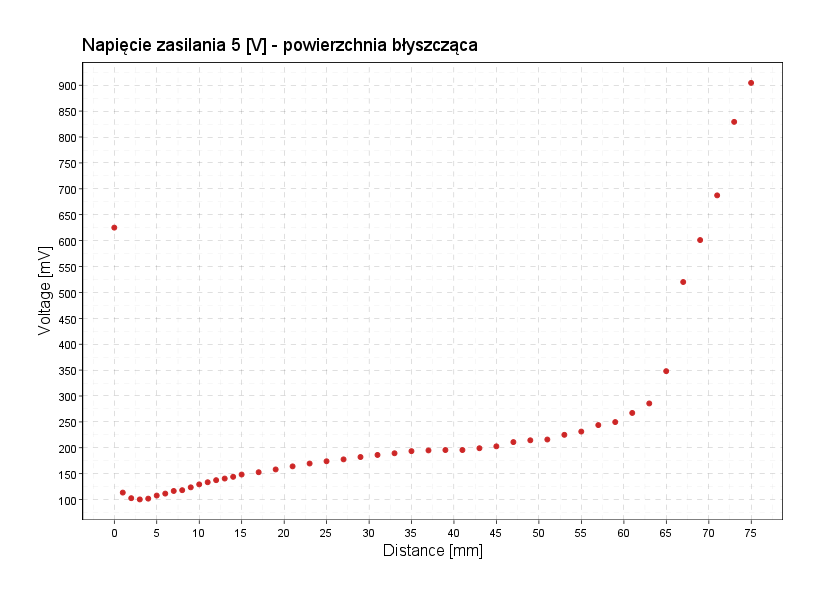
\includegraphics[scale = 0.5]{F:/Projekty Intellij/Text/Metrologia/Ćwiczenie8/Img/RplotRef5Full.png}
    \end{center}
    \par Producent podaje że czujnik poprawnie rejestruje odległość w zakresie od 0.2 do 15 [mm] z uwagą że pomiar odbywa się w atmosferze pozbawionej światła zewnętrznego.
    Na wykresie zauważamy że czujnik zaczyna poprawnie mierzyć powyżej dystansu 2 [mm]. Może to być związane z wpływem światła otocznia na pomiar a dla pomiaru przy odległości 0 [mm]
    z braku miejsca dla czujnika na odbicie wiązki światła i odebrania jej. Dla tego prawdopodobnie zakres podany od producenta nie zaczyna się od wartości 0 gdyż producent zdaje sobie
    sprawę z tego zjawiska. Idąc dalej widzimy że
    rzeczywiście charakterystyka czujnika do odległości 15 [mm] zachowuje się liniowo a przy dalszych pomiarach zaczyna powoli się zmieniać. Najciekawsze zjawiska zachodzą przy odległości
    około 35 - 40 [mm] gdzie charakterystyka zaczyna się wypłaszczać oraz powyżej odległości 60 [mm] gdzie charakterystyka zaczyna gwałtownie rosnąć.\\
    \indent Dla zakresu poprawnego działania czujnika (w tym przypadku od 3 do 15 [mm]) wyznaczono approksymację liniową danych oraz wyliczono
    współczynnik determinacji $R^2$ dla tej funkcji:
    \begin{center}
        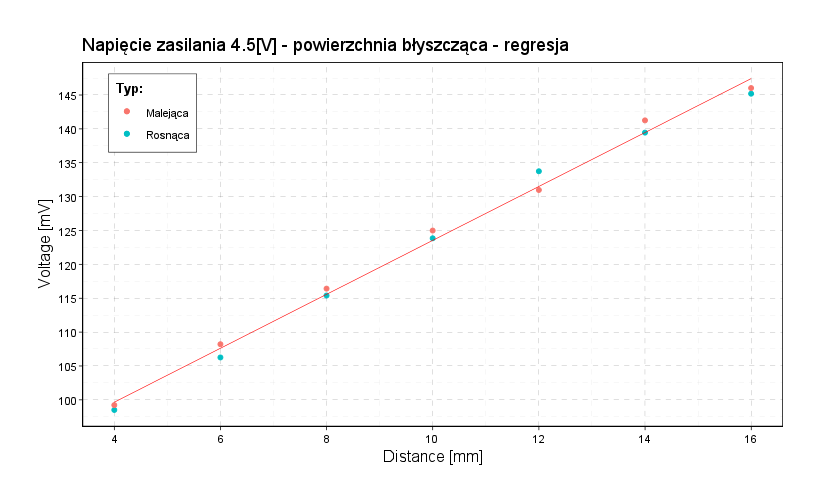
\includegraphics[scale = 0.5]{F:/Projekty Intellij/Text/Metrologia/Ćwiczenie8/Img/RplotregresjaDistance.png}
    \end{center}
    \begin{gather*}
        R^2=0.9964
    \end{gather*}
    \indent Można zauważyć że współczynnik determinacji ma wartość powyżej 99.5 [\%] co oznacza bardzo dokładne przybliżenie do funkcji
    liniowej która aproksymowała dane.\\
    \indent Czułość lokalna czujnika wyznaczono ze wzoru:
    \begin{gather*}
        S=\frac{\Delta Y}{\Delta X}
    \end{gather*}
    \indent Czułości dla kolejnych pomiarów została wyznaczona dla miejsc w odległości 6 , 10 i 14 [mm] od czujnika:
    \begin{center}
        \csvreader[tabular = |c|c|c|c|,
            table head = \hline  \textbf{Typ próby} & \textbf{\boldmath$S_6$[$\frac{V}{mm}$]} & \textbf{\boldmath$S_{10}$[$\frac{V}{mm}$]}
            & \textbf{\boldmath$S_{14}$[$\frac{V}{mm}$]} \\\hline,
            late after line = \\\hline
        ]{Dane/Sensitivity.csv}{}{
                \csvcoli & \csvcolii & \csvcoliii & \csvcoliv
        }
    \end{center}
    \par Na podstawie czułości dla serii o napięciu zasilania 4.5 [V] i błyszczącej powierzchni odbijającej wyznaczono kolejne 10 wartości jakie
    przyjmują charakterystyki dla różnych czułości. Wartości te wyliczono w zakresie od 4 do 40 [mm] i porównano je ze średnią z pomiaru właściwego.
    Dane zostały przedstawione na wykresie poniżej:
    \begin{center}
        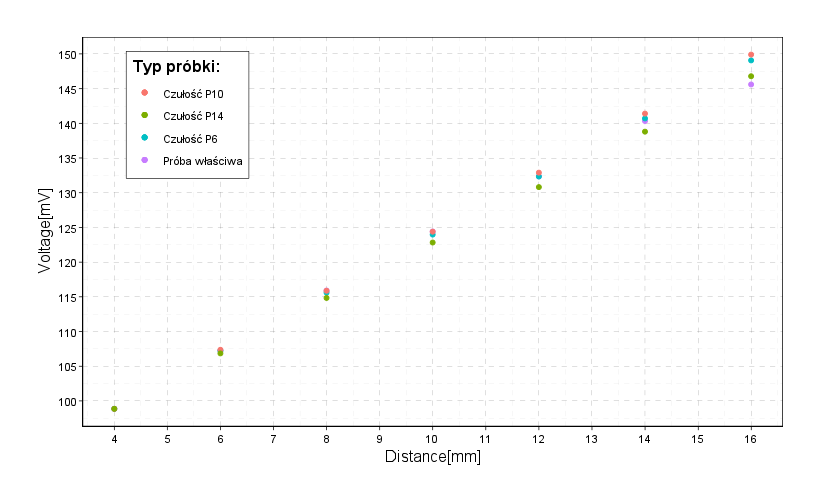
\includegraphics[scale = 0.5]{F:/Projekty Intellij/Text/Metrologia/Ćwiczenie8/Img/RplotNoise.png}
    \end{center}
    \par Można zauważyć że wartości są bardzo zbliżone w zakresie pracy miernika ale rozbiegają się od wartości zmierzonej gdy przekroczą zakres
    pomiarowy czujnika. Pokazuje to dobrze dlaczego zakres ten jest tak mocno ograniczony. Poniżej przedstawiono dodatkowo powyższy wykres
    ale ograniczony jedynie do zakresu pomiarowego czujnika:
    \begin{center}
        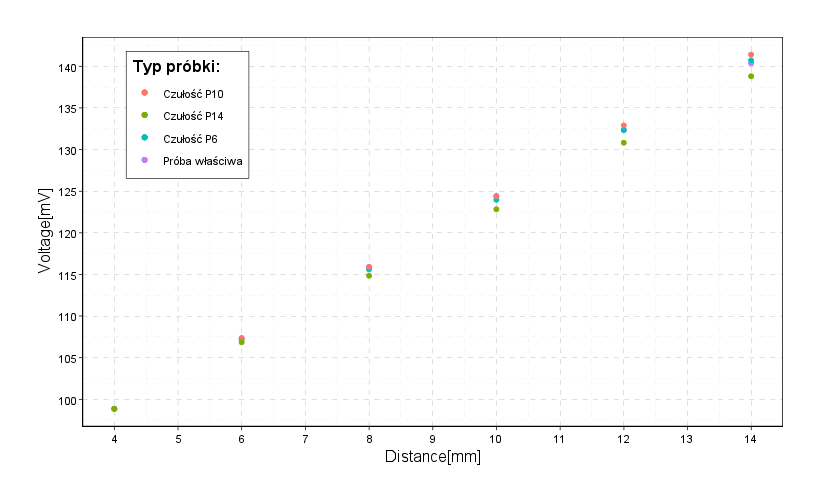
\includegraphics[scale = 0.5]{F:/Projekty Intellij/Text/Metrologia/Ćwiczenie8/Img/RplotNoise2.png}
    \end{center}
    \par Z powodu braku informacji na temat wyznaczania przedziału szumowego w wstępie teoretycznym oraz w otwartych źródłach zewnętrznych
    wartości przedziału szumowego zostały wyznaczone autorską metodą. Przedział szumowy wyznaczono na podstawie wartości przy zmiennej rosnącej
    oraz malejącej dla histerezy pomiaru odległości. Przedziału szumowego wyznacznao dla pomiaru przy zasilaniu 5 [V] oraz dla błyszczącej powierzchni
    odbijającej. Wartość szumu wyznaczono jako średnią wartość z różnicy między wartością malejącą oraz rosnącą charakterystyki czujnika. Wartość
    wyznaczono jedynie dla danych z przedziału poprawnego działania czujnika, w tym przypadku od 3 do 15 [mm]. Wyznaczono stały przedział
    szumu na wartość: $N_{Int}=\pm 290.5769 [\mu V]$ od wartości średniej z serii rosnącej oraz malejącej charakterystyki.\\
    \indent Na podstawie powyższej wartości przedziału szumu możemy wyznaczyć rozdzielczość czujnika przy użyciu wzoru:
    \begin{gather*}
        Res=\frac{\Delta X\cdot N_{Int}}{\Delta Y}
    \end{gather*}
    Po podstawieniu wartości otrzymujemy:
    \begin{gather*}
        Res=\frac{(15[mm]-3[mm])\cdot 0.00058[V]}{0.147865[V]-0.100335[V]}\approx 0.15[mm]
    \end{gather*}
    Teoretycznie więc przy użyciu tego czujnika można byłoby mierzyć z rozdzielczością 0.15[mm].
    \par Dla czujnika wyliczono selektywność pomiarową na podstawie pomiaru z matową powierzchnią i przy różnicy napięcia
    zasilania od rzeczywistego równej 0.5[V]. Wykorzystano do tego wzór:
    \begin{gather*}
        \sigma=\frac{\Delta Y}{Y\cdot \Delta Z}=\frac{\Delta Y_5 - \Delta Y_{4.5}}{\Delta Y_{4.5} \cdot \Delta Z}
    \end{gather*}
    Uzyskano na tej podstawie wynik:
    \begin{gather*}
        \sigma=0.0099 [\frac{\%}{mV}]
    \end{gather*}


    \subsection*{Czujnik natężenia światła - fotorezystor i dioda}
    Na podstawie danych zgromadzonych w trakcie przebiegu doświadczenia wyznaczono wykresu zależności napięcia na wyjściu czujnika od poziomu szarości
    powierzchni naświetlanej:
    \begin{center}
        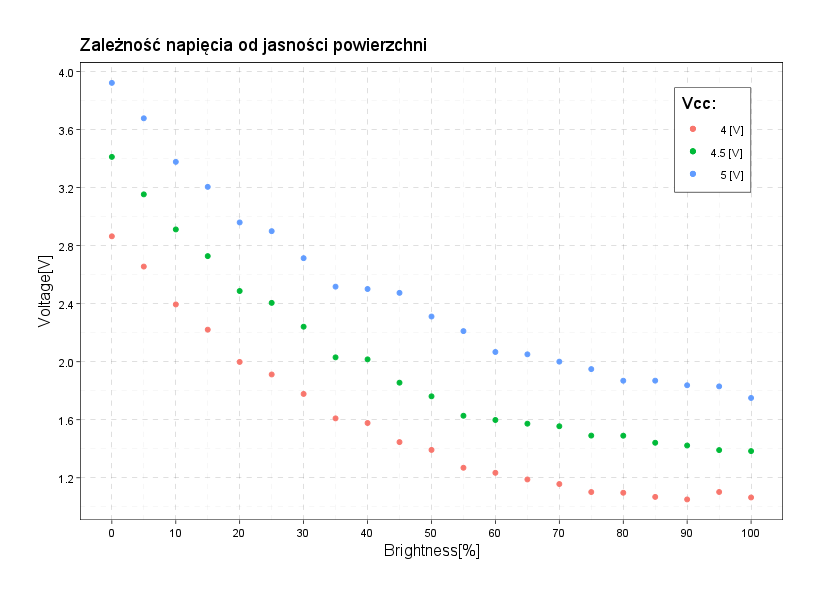
\includegraphics[scale = 0.5]{F:/Projekty Intellij/Text/Metrologia/Ćwiczenie8/Img/RplotBright.png}
    \end{center}
    \par Na podstawie wykresu jesteśmy w stanie zauważyć że charakterystyka powyższej zależności nie jest charakterystyką liniowa a przypomina bardziej
    funkcję hiperboliczną. Wykorzystując regresję liniową zaproksymowano krzywą dla napięcia zasilania równego 5 [V]. Z aproksymacji uzyskano krzywą
    której współczynnik determinacji $R^2$ względem danych pomiarowych wynosił 0.9107. \\
    \indent Z powodu braku charakterystyki malejącej czujnika nie jesteśmy w stanie podać parametrów szumowych. Rozdzielczość pomiarowa tego czujnika
    na podstawie doświadczenia to conajmniej 5 [\%] zmiany jasności powierzchni gdyż dla takiej najmniejszej zmiany wykonywano kolejne pomiary.\\
    \indent Selektywność w odniesieniu do napięcia zasilania dla napięcia zasilania 4.5 [V] wynosi:
    \begin{gather*}
        \sigma=14.20[\frac{\%}{V}]
    \end{gather*}

    \subsection*{Czujnik tętna}
    Na podstawie obserwacji zmian sygnału na wyjściu czujnika przy pomocy oscyloskopu wyznaczono: częstotliwość sygnału oraz okres.
    Korzystając z poniższych wzorów wyznaczono tętno:
    \begin{gather*}
        BPM=f\cdot 60=\frac{60}{T}
    \end{gather*}
    Uzyskano tętno równe:
    \begin{gather*}
        BPM=83.34 [BPM]
    \end{gather*}
    Poniżej przedstawiono zarejestrowany przebieg:
    \begin{center}
        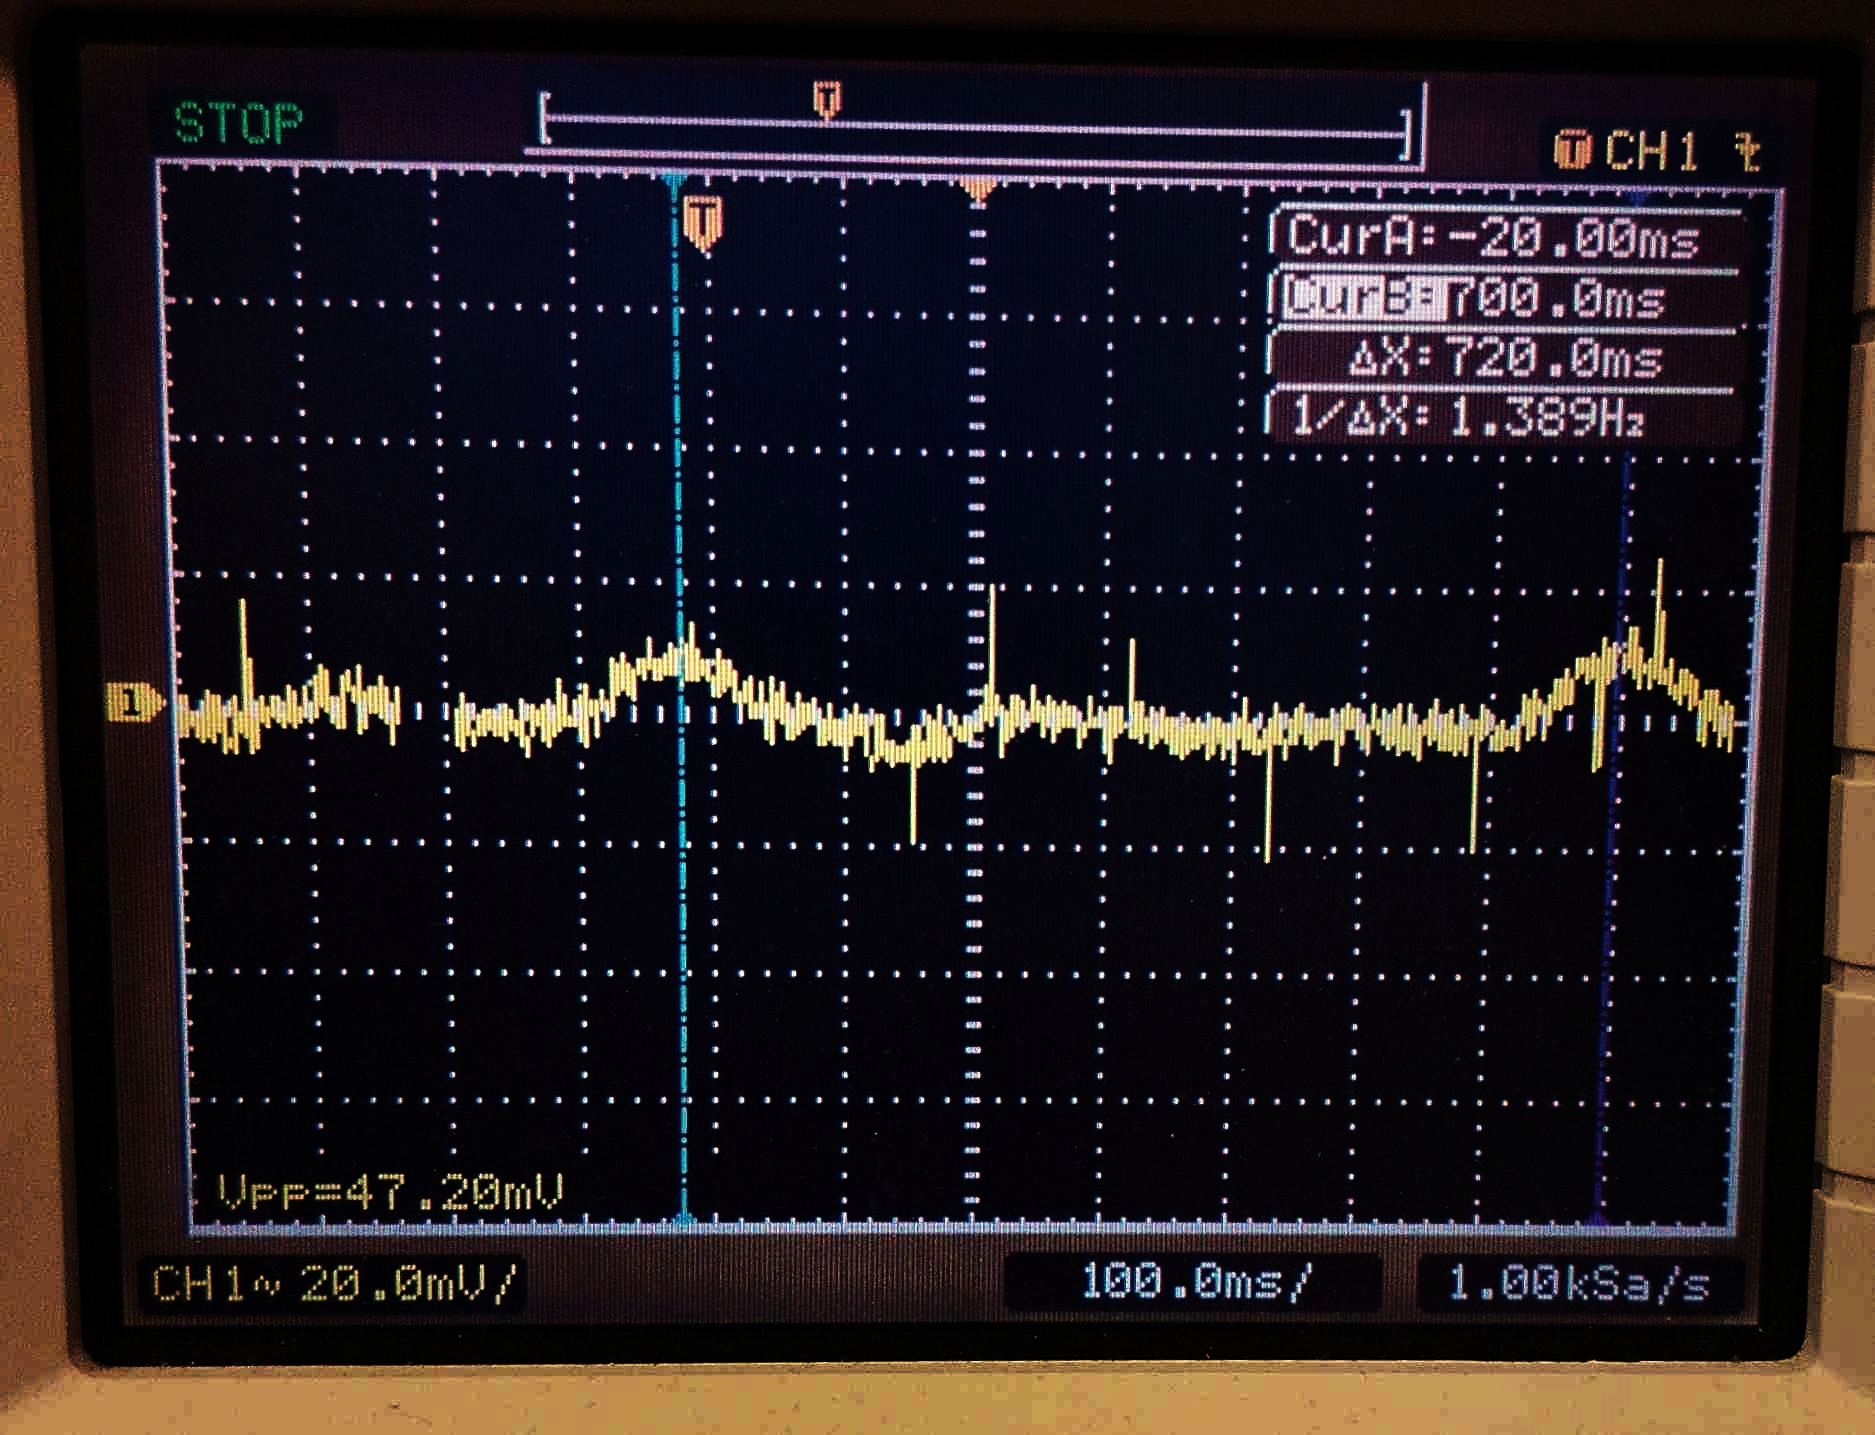
\includegraphics[scale = 0.23]{F:/Projekty Intellij/Text/Metrologia/Ćwiczenie8/Img/img.png}
    \end{center}

    \section{Uwagi i wnioski}
    Z pomiarów obejmujących czujnik odległości TCRT5000 możemy empirycznie zauważyć pełną charakterystykę czujnika
    również poza zakresem działania czujnika. Wnioski na temat pełnej charakterystyki czujnika znajdują się w części 4.
    Możemy zauważyć że funkcjonowanie czujnika jest bezpośrednio skorelowane z napięciem zasilania. Już spadek napięcia o 0.5 [V] potrafi obniżyć amplitudę
    sygnału wyjściowego oraz zmniejszyć zakres działania. Największy wpływ na funkcjonowanie czujnika miała powierzchnia odbijająca. W przypadku powierzchni
    błyszczącej czujnik podawał informacje zwrotne nawet do odległości 100 [mm]. Jednak przy powierzchni matowej ta wartość spadła o połowę przy napięciu zasilania
    równym 5 [V] a przy napięciu zasilania równym 4 [V] spadła do długości zaledwie 40 [mm].\\
    \indent Na podstawie wykresów przedstawiające pętle histerezy w zakresie działania czujnika można zauważyć że pętla histerezy nie jest spójna z założeniami teoretycznymi.
    Dla niektórych pomiarów charakterystyka malejąca zamieniała się miejscem z charakterystyką rosnącą. Wynika to prawdopodobnie z bardzo małej dokładności samego doświadczenia.
    Instrumenty wykorzystane do określania odległości i ich tolerancje nie pozwalały na dokładne określenie odległości ani na stabilne przytrzymanie powierzchni odbijającej w punkcie
    pomiarowym. Doświadczenie można poprawić wykorzystując sztywny liniał metalowy oraz element odbijający który sztywno trzyma się w liniale oraz pozwala na blokowanie pozycji.\\
    \indent W przypadku wyznaczanie szumów oraz rozdzielczości miernika należy pamiętać że do pomiaru wykorzystujemy linijkę posiadającą dokładność 1 [mm] oraz to że dokładność
    samego eksperymetnatora nie jest zerowa. Można więc wywnioskować że rozdzielczość zmierzona będąca mniejszą od tej niepewność nie będzie wartością rzeczywistą. Również
    zastosowane w obliczeniach przedziału szumowego założenie że przedział ten ma stałą wartość jest nieprawdziwe. Z samej pętli histerezy wynika że przedział ten jest szerszy w połowie
    przedziału pracy czujnika a najwęższy przy jego krańcach.\\
    \\
    \indent Dla czujnika barw zauważono po pierwsze że nie każda charakterystyka przetwornika jest charakterystyką liniową. Nie pozwala to często na bezpośredni odczyt
    wartości mierzonej i wymaga układu kondycjonującego zamieniający charakterystykę nieliniową na liniową. Tak jak dla poprzedniego czujnika zaobserwowano spadek amplitudy
    sygnału przy zmianie napięcia zasilania. Dla najniższego napięcia zasilania 4 [V] można zauważyć że powyżej wartości 80 [\%] szarości, kolejne pomiary zaczynają
    przyjmować charakterystykę liniową. Powoduje to brak możliwości rozróżnienia tych wartości od siebie. Raz jeszcze więc warto zaznaczyć jak kluczowe do poprawnego działania
    przetworników jest stabilne napięcie zasilania o właściwych parametrach.\\
    \\
    \indent Dla czujnika tętna można zauważyć na podstawie przebiegu na oscyloskopie bardzo duże zaszumienie sygnału wysokimi częstotliwościami. Idealnym więc byłoby zastosowanie
    opowiedniego filtra dolnoprzepustowego w celu odfiltrowania szumu od właściwego sygnału. Amplituda sygnału również nie jest wysoka więc bardzo dobrym usprawnieniem czujnika
    byłoby dodanie odpowiedniego układu wzmacniającego sygnał. Na sygnale również widać pojedyncze impulsy o charakterystyce delty Diraca. Impulsy te posiadają amplitudę
    o większej wartości niż interesujące nas okresowe wzgórza właściwego sygnału. Mogą one mieć szkodliwe działanie na dalsze układy pomiarowe wykorzystujące sygnał do
    wyznaczania np.: wartości tętna.

    %Bibliografia
    \vfill
    \footnotesize
    \begin{thebibliography}{3}
        \bibitem{texbook1}
        https://wzn.pwr.edu.pl/materialy-dydaktyczne/metrologia-elektroniczna
        \bibitem{texbook2}
        https://www.vishay.com/docs/83760/tcrt5000.pdf
        \bibitem{texbook3}
        http://elektron.pol.lublin.pl/elekp/\_wyklad\_PWN/E\_Pawlowski\_wyklad\_PWN\_EMST\_2019\_w02.pdf
    \end{thebibliography}
\end{document}